%\documentclass[11pt]{article}
\documentclass{icldt}
%============================================================
% Don't touch this
% Preamble 
%\usepackage[a4paper, inner=1.5cm, outer=2.5cm, top=1.5cm,bottom=2.5cm, bindingoffset=1cm]{geometry} 
\department{Mechanical Engineering}
\supervisor{Ambrose Taylor}

%----------------------------------------------------------------------------
% Inserting Important Packages
\usepackage[english]{babel}
\usepackage{graphicx}
\usepackage{amsmath}
\usepackage{epstopdf}
\usepackage{bbm} 
\usepackage{rotating}
\usepackage{mathtools}
\usepackage{verbatim}
\usepackage{placeins}
\usepackage{textgreek}
\usepackage{fixmath}
\usepackage{varioref}
\usepackage[pdftex,bookmarks=true,hidelinks]{hyperref}
\usepackage{cleveref}
\usepackage{lineno}
\usepackage{amssymb}
\usepackage{tabularx}
\usepackage{array}
\usepackage{lscape}
\usepackage{pdflscape}
\usepackage{xr}
\usepackage{caption}
\usepackage{subcaption}
\usepackage{multirow}
\usepackage{pdfpages}
\usepackage{mathrsfs}
\usepackage{notoccite}
\usepackage{enumitem}
%\usepackage[intoc]{nomencl}
\newcommand{\HRule}{\rule{\linewidth}{0.5mm}}


%============================================================

\begin{document}
\Crefname{equation}{Eq.}{Eqs.} % this is to change the equation number style
%===============================
% Title Page
\title{Put Title Here}
\author{Your name}
\date{\today}
%\begin{center}
%\textsc{\LARGE Final Report}\\[1.5cm]
%% Title
%\HRule \\[0.4cm]
%{ \large \bfseries  Title Here}\\[0.4cm]
%\HRule \\[1cm] 
%{\large \today} \\[1.5cm] 
%% Author and supervisor
%\begin{minipage}{0.4\textwidth}
%\begin{center} \large
%\emph{Author:}\\
%Junyi \textsc{Lee}
%\end{center}
%\end{minipage}
%\end{center}

\pagenumbering{gobble} 
\maketitle
\newpage

%===============================

% Abstract
\pagenumbering{roman}
\section*{Abstract}
\addcontentsline{toc}{section}{Abstract}

This is where you type the abstract.

\newpage
%======================
% Table of contents
\tableofcontents
\newpage
\listoftables
\newpage
\listoffigures

\newpage
\pagenumbering{arabic}
%=============================

% Text Starts here
\chapter{First Chapter}
\section{Introduction}

Please find the template for citing stuff here. The figure is shown in \Cref{MyFigure}. 

% This is a figure
\begin{figure}[!htpb]
\centering
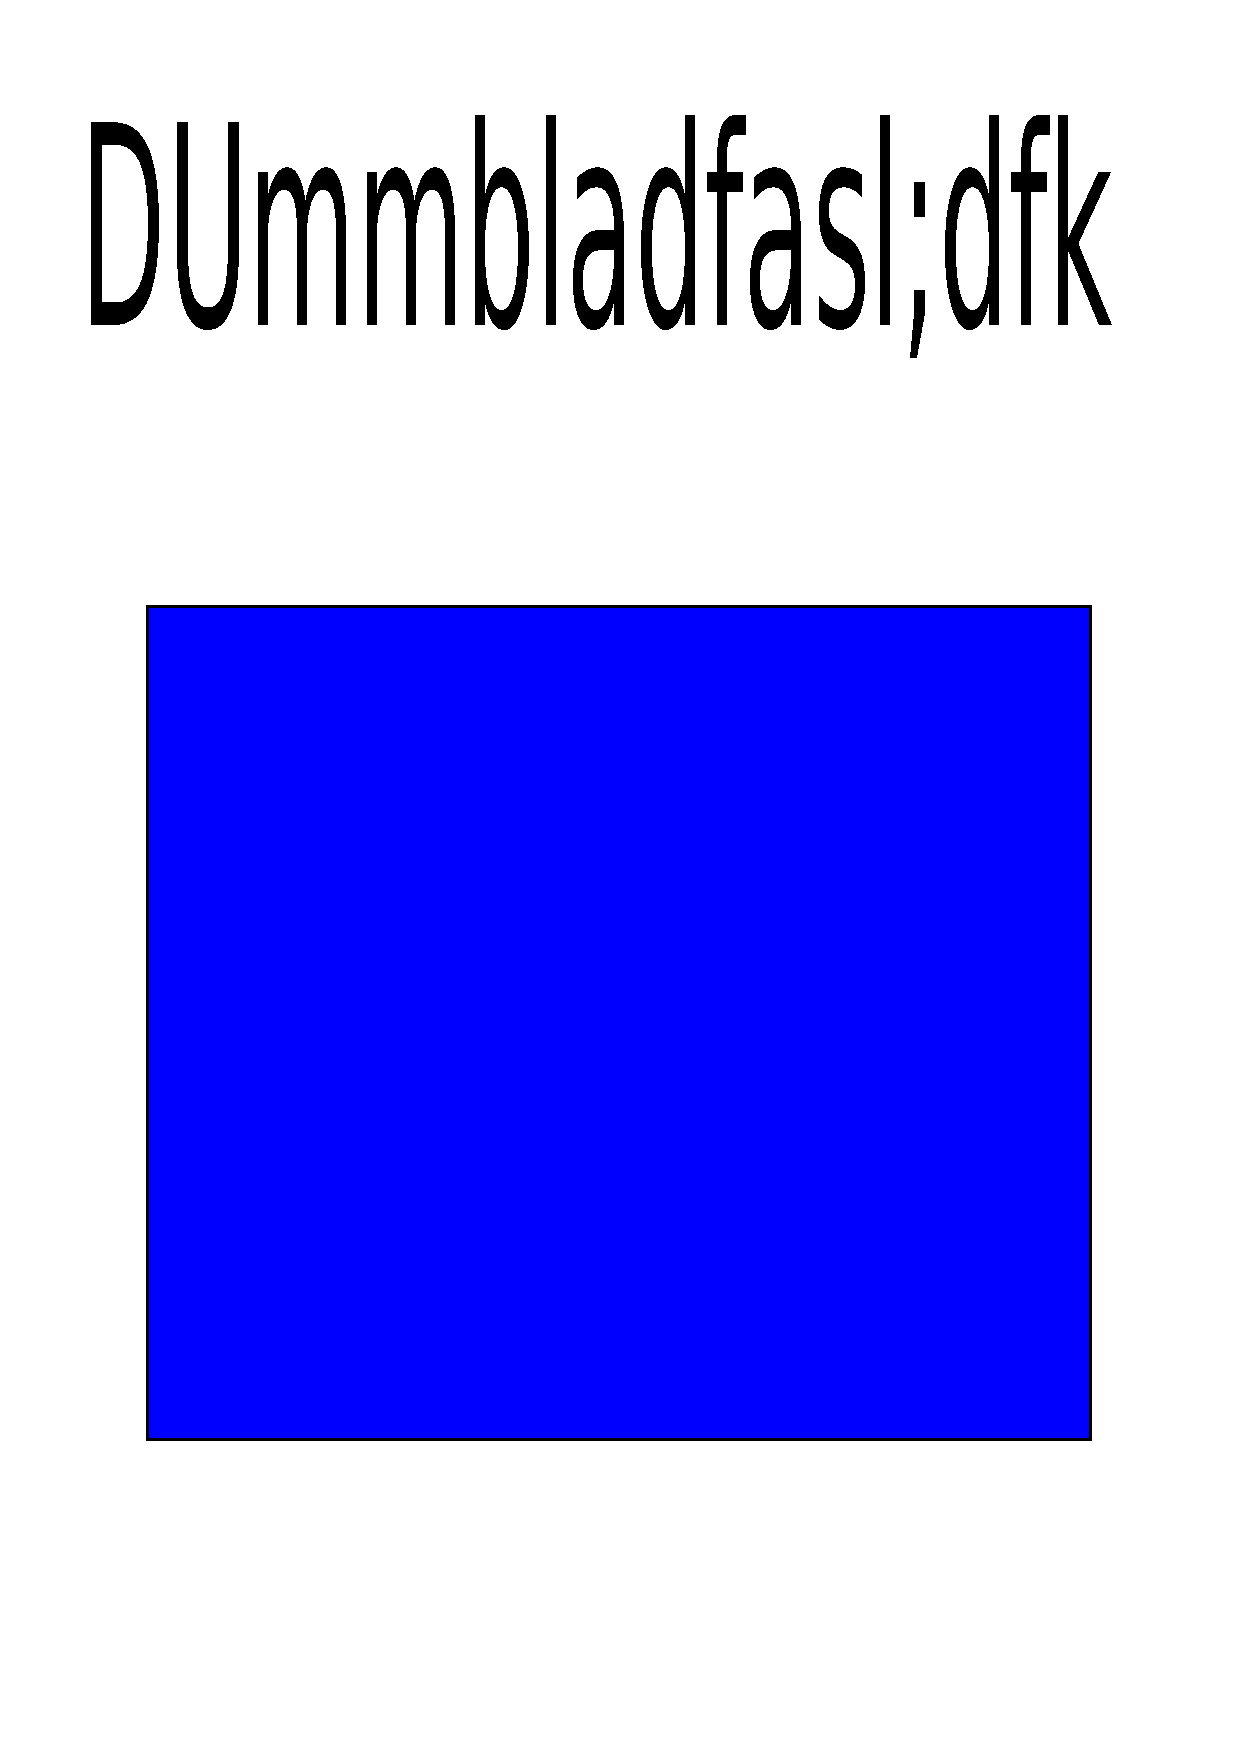
\includegraphics[height=8cm]{dummypic}
\caption{A Figure} \label{MyFigure}
\end{figure}

\Cref{MyFigure} is shown above

\FloatBarrier % this command blocks the figure from going over this part

\subsection{My Subsection 1}
Just refer to \Cref{MyTable}

% This is a table
%====================
\begin{table}[htbp]
\begin{tabular}[htbp]{|c|l|}
\hline
Number Stored & Description\\
\hline
Content 1 & Content 2 \\
\hline
\end{tabular}

\caption{My Table Caption} \label{MyTable}
\end{table}
%====================

\subsection{My Subsection 2}
Now there are two ways to type equation one is $e=mc^2$ or $\text{e} = \text{mc}^2$ The other see \Cref{MyEq1}. This is the reference \cite{RN2}

\begin{equation} \label{MyEq1}
\frac{Numerator}{Denominator} \left( \sigma \right)
\end{equation}

\section{Second section}
This is the second section

\chapter{Second Chapter}
This is the second chapter test
%=============================================
% This is the bibliography
\bibliographystyle{ieeetr} % This is the style
\addcontentsline{toc}{section}{References} % This is to say that 
\bibliography{ReferenceLibrary}

%=============================================
% This is the Appendix
\FloatBarrier
\newpage
\appendix
\chapter{Appendices}
This is the appendix
\section{Input file-TDCB model}
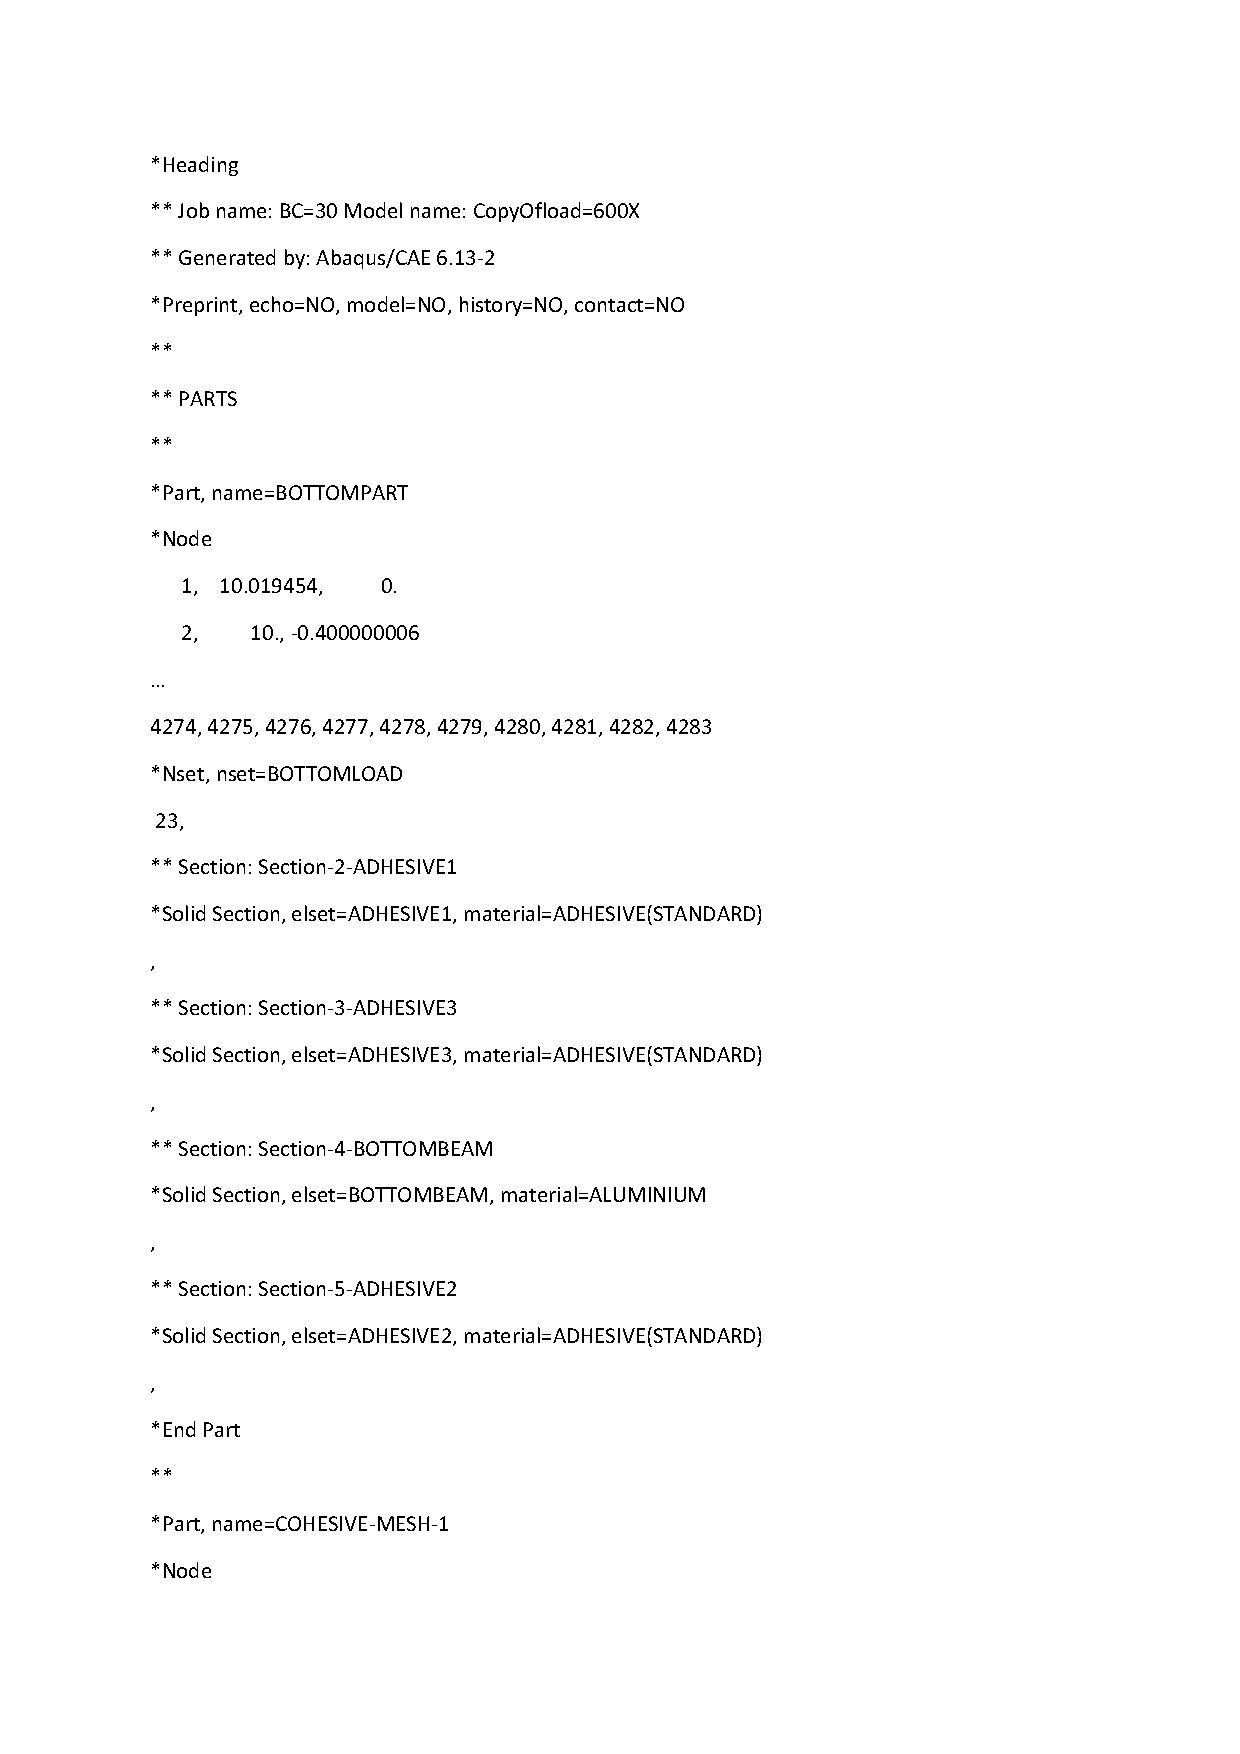
\includepdf[pages=-]{inputFile1.pdf}
\end{document}